\section{Probabilità sulla retta reale}
In questo paragrafo vedremo due classi principali di esempi di probabilità su $\Omega = \R$.
Queste due classi non esauriscono i possibili esempi di probabilità su $\R$ ma saranno l'oggetto
delle applicazioni che vedremo.

\subsection{Probabilità discreta}
Una \textbf{probabilità discreta} su $\Omega = \R$ è una probabilità su $\Omega = \R$, prendendo
come $\sigma$-algebra le parti di $\R$ ($\F (\mathcal{P}(\R))$), che sia \textbf{concentrata} su
una successione finita o numerabile $x_1, x_2, \dots$ di punti.

Ad esempio la probabilità associata al numero di volte che esce testa in due lanci di moneta è
una probabilità discreta, concentrata su $\{0,1,2\}$. Infatti abbiamo che per due lanci di moneta
i possibili esisti sono
\[ \Omega = \{ (0,0), (0,1), (1,0), (1,1) \} \]
Come possiamo vedere in un solo caso non esce testa, in due casi esce solo una testa e in un solo
caso esce due volte testa.

\begin{center}
	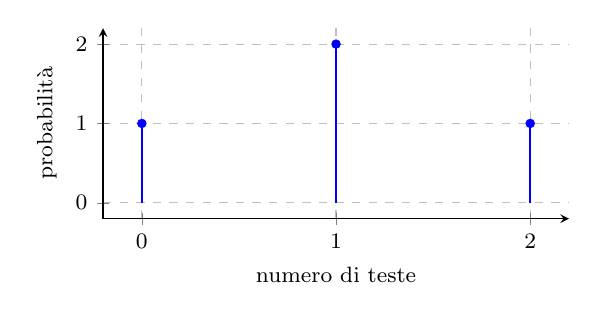
\begin{tikzpicture}
		\begin{axis}[
				font=\footnotesize,
				width=7.5cm,
				height=4cm,
				axis lines = left,
				xlabel = numero di teste,
				ylabel = probabilità,
				xtick = {0, 1, 2},
				ytick = {0, 1, 2},
				ymin = 0, ymax = 2,
				xmin = 0, xmax = 2,
				grid = both,
				grid style = dashed,
				legend pos = north west,
				enlargelimits
			]

			\draw [thick, blue] {(0, 0) -- (0, 1)};
			\draw [thick, blue] {(1, 0) -- (1, 2)};
			\draw [thick, blue] {(2, 0) -- (2, 1)};
			\filldraw[blue] (0, 1) circle (1.5pt);
			\filldraw[blue] (1, 2) circle (1.5pt);
			\filldraw[blue] (2, 1) circle (1.5pt);
		\end{axis}
	\end{tikzpicture}
\end{center}

Sia $p_i = p(x_i) = P(x_i)$ la probabilità che $x_i$ si verifichi e sia $A \subseteq \Omega$
il sottoinsieme di eventi $x_i$, allora vale che
\begin{equation}\label{eq: 3.1}
	P(A) = \sum_{x_i \in A} p(x_i)
\end{equation}

\begin{definition}
	La funzione
	\[ p : \R \to [0,1] \]
	si dice \textbf{funzione di massa} o \textbf{densità discreta} di $P$. Essa è definita in modo
	da assumere valore 0 per eventi non presenti all'interno di $\Omega$. Vale infatti
	\[
		p(x) = \begin{cases}
			P(\{ x \}) & x \in \Omega    \\[1ex]
			0          & x \notin \Omega
		\end{cases}
	\]
\end{definition}

Per adesso non stiamo dicendo nulla di molto diverso rispetto a quanto detto sulla probabilità e
le sue proprietà. Stiamo però fornendo un modo per modo per visualizzare la probabilità e come
essa è distribuita sulla retta reale $\R$. La funzione di massa non fa altro che associare ad
ogni evento dello spazio campionario una probabilità, associa invece probabilità nulla ad eventi
non presenti nello spazio campionario.

\begin{observation}
	Facciamo ora alcune osservazioni:
	\begin{itemize}
		\item La probabilità $p$ soddisfa
		      \[ p(x_i) \geq 0 \quad \land \quad \sum_i p(x_i) = P(\R) = 1 \]
		\item Viceversa, data una successione $x_1, x_2, \dots$ finita o numerabile e una funzione
		      $p$ con le proprietà descritte sopra, allora esiste un'unica probabilità $P$ su $\R$
		      avente $p$ come funzione di massa.
		\item Dalla formula \ref{eq: 3.1}, è possibile calcolare $P(A)$ partendo dalla successione
		      degli $x_i$ e dalla funzione di massa.
	\end{itemize}
\end{observation}

\subsection{Probabilità con densità}
Vogliamo ora descrivere come la probabilità viene distribuita in spazi campionari continui. Per
farlo dobbiamo definire gli strumenti necessari ad operare su tali spazi campionari.

\begin{theorem}
	Esiste una $\sigma$-algebra $\F \subset \mathcal{P}(\R)$ tale che
	\[ (a, b) \in \F \]
	con $-\infty \leq a < b \leq +\infty$ ed esiste
	\[ \lambda : \F \to [0, +\infty) \]
			che sia $\sigma$-additiva e tale che, per ogni $-\infty \leq a < b \leq +\infty$ vale
			\[ \lambda((a,b)) = \lambda((a,b]) = \lambda ([a,b)) = \lambda([a,b]) = b - a \]
\end{theorem}

Chiameremo gli elementi di $\F$ \textbf{insiemi misurabili}. Intersecando tutti gli elementi di
$\F$ con l'intervallo $[0,1]$ otteniamo i sottoinsiemi misurabili di quest'ultimo, che sono una
$\sigma$-algebra sulla quale possiamo definire la probabilità
\[ P (A) = \lambda (A) \]
per ogni $A \subset [0,1]$ misurabile, in modo che
\[ P((a, b)) = |b - a| \]
per ogni $a,b \in [0,1]$.

\begin{observation}
	Osserviamo che $\lambda$ assegna lunghezza nulla ai singoli punti, ovvero
	\[ \lambda(x) = \lambda([x,x]) = x - x = 0 \]
	e lo stesso vale per ogni sottoinsieme $A \subset \R$ con al più numerabili elementi.
\end{observation}

\begin{definition}
	Si chiama \textbf{densità di probabilità} sulla retta reale, una funzione non negativa
	$f : \R \to [0, +\infty)$, integrabile e tale che
	\[ \int_{-\infty}^{+\infty} f(x) dx = 1 \]
	Ad ogni densità di probabilità si associa un'unica probabilità sulla $\sigma$-algebra degli
	insiemi misurabili di $\R$ definita da:
	\[ P(A) = \int_A f(x) dx \]
	per ogni $A \in \F$.
\end{definition}

Perché questa sia una buona definizione si deve controllare che $P$, così definita, soddisfi
\[ P(\R) = \int_\R f(x) dx = 1 \]
per ipotesi, ed inoltre se $A \cap B = \emptyset$ si ha che
\[ P(A \cup B) = \int_{A \cup B} f(x) dx = \int_A f(x) dx + \int_B f(x) dx = P(A) + P(B) \]
Se $X$ ha densità $f$, allora vale
\[ P(X = t) = P_X (t) = \int_{\{t\}} f(x) dx = 0 \]
per ogni $t \in \R$.